\section{Pruebas llevadas a cabo} \label{sec:pru}
% describiranse as probas realizadas aos distintos niveis para
% garantir o correcto funcionamento do software ou do hardware.
    
    Muchos de los paradigmas de programación ágil abarcan el concepto de prueba unitaria. Pruebas programadas en el mismo lenguaje que se escribe la aplicación y que permiten comprobar el funcionamiento de una unidad de código. Sin embargo, dado que desde el inicio del proyecto no estaban claras las fuentes de información que iban a ser utilizadas debido a la gran variedad de librerías y las diferencias entre estas, además de la posibilidad de adición de cambios en el proyecto que pudiesen suponer una modificación de toda su estructura y funcionamiento, se tomó la decisión de no utilizar pruebas automatizadas.
    
    \subsection{Pruebas generales de funcionamiento}
        Para comprobar el correcto funcionamiento del sistema se decidió realizar pruebas manuales, comprobando con cada cambio las funcionalidades previamente desarrolladas e introduciendo valores correctos e incorrectos en los campos a comprobar.
        
        Para detectar el éxito o fallo de las pruebas realizadas se utilizó la consola de comandos, mostrando allí el resultado obtenido en cada ejecución, este mecanismo de pruebas ayudaría a desarrollar una base del sistema, es decir, alcanzar un punto donde el agente fuese capaz de gestionar correctamente los diferentes \textit{plugins} y hacer uso de estos a través de la \textit{CLI}.
        
    \subsection{Pruebas de funcionamiento como servicio}
        El mecanismo mencionados anteriormente es útil durante el desarrollo de de las funcionalidades principales, sin embargo, probar el servicio supone una tarea más complicada ya que no es posible mostrar la información en la línea de comandos.
        
        Para comprobar la ejecución del agente al ser utilizado como servicio se decidió utilizar dos métodos, comprobar los sistemas remotos a donde se envía la información para determinar si llega correctamente y los \textit{eventos del sistema} donde se muetra cualquier información relacionada con el agente en sí.
        
        El desarrollo de un sistema de actualización automática ayudó con las pruebas mencionadas en este apartado, ya que eliminaó la necesidad de reiniciar el servicio manualmente y de copiar nuevas versiones de los \textit{plugins} para realizar cada prueba.
    
    \subsection{Pruebas de actualización automática}
        Para comprobar que el sistema de actualización automática funcionara correctamente se utilizaron los \textit{eventos del sistema}, donde fueron añadidos \textit{logs} para cada acción realizada, como la actualización de algún componente, cualquier tipo de fallo, o un indicador de que el proceso de actualización había terminado.
        
    \subsection{Eventos del sistema}
        Cada \textit{log} creado por el agente o el sistema de actualización automática cuenta con un identificador de evento que permite saber de dónde proviene el mensaje recibido. En el anexo \ref{anx:eventid} se muestra una lista con los identificadores para cada uno de los procesos.
        
    \subsection{Resultados obtenidos}
        En las figuras \ref{fig:rabbitmq-prod-queue} y \ref{fig:rabbitmq-dev-queue} se muestran las colas de dos servidores de \textit{RabbitMQ} (producción y desarrollo), donde se pueden apreciar los resultados de la ejecución como servicio en uno de los servidores \textit{Windows} del \textit{CERN} durante varios días. La configuración utilizada incluye más \textit{plugins} de los inicialmente planteados para este proyecto (\textit{HeartBeat} y \textit{Updates}), los cuales se han mantenido en ejecución por más de una semana.
        
        \begin{figure}[h!]
        \centering
            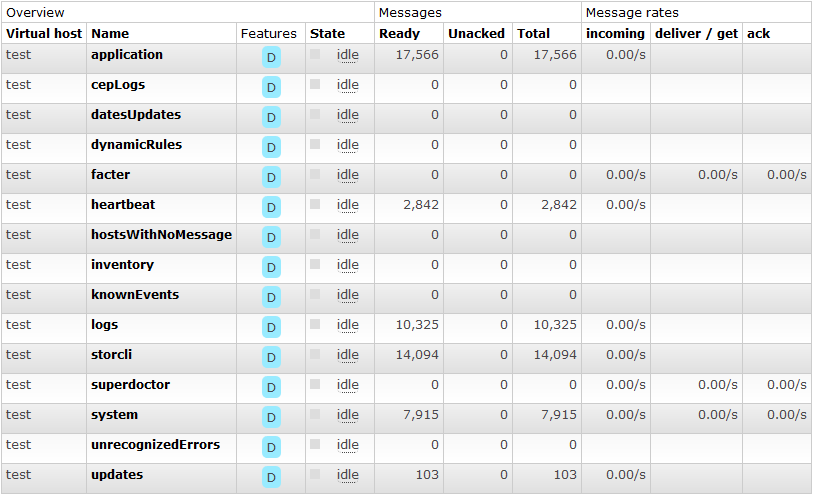
\includegraphics[scale=0.8]{cola-rabbit-mq-prod.png}
            \caption{Colas de RabbitMQ - Producción}
            \label{fig:rabbitmq-prod-queue}
        \end{figure}
    
        \begin{figure}[h!]
        \centering
            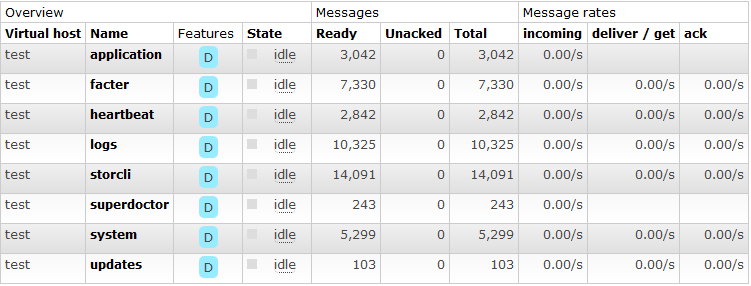
\includegraphics[scale=0.9]{cola-rabbit-mq-dev.png}
            \caption{Colas de RabbitMQ - Desarrollo}
            \label{fig:rabbitmq-dev-queue}
        \end{figure}
        
        Las columnas mostradas brindan información acerca del estado de las colas, a continuación se da una breve descripción de cada una.
        
        \begin{itemize}
            \setlength\itemsep{2em}
            \item \textbf{VirtualHost:} Grupo lógico de entidades al que pertenece la cola. \cite{virtualhost}
            \item \textbf{Name:} Nombre de la cola que recibe la información
            \item \textbf{Features:} Configuración de la cola, la ``D'' significa que la cola está marcada como ``durable'', es decir, que los mensajes persisten en la cola hasta que se indique lo contrario.
            \item \textbf{Status:} Estado de la cola, indica si está libre o recibiendo mensajes en ese momento.
            \item \textbf{Ready:} Número de paquetes disponibles para ser consumidos.
            \item \textbf{Unacked:} Número de mensajes que fueron consumidos y de los que no se recibió confirmación.
            \item \textbf{Total:} Total de mensajes recibidos.
        \end{itemize}{}
        
        Estas imágenes demuestran que hay datos llegando a los servidores \textit{RabbitMQ}, sin embargo, el número de horas de ejecución del agente no coincide con la cantidad de paquetes recibidos para ambos \textit{plugins}. Esto se debe a que la información almacenada en estos servidores incluye mensajes de pruebas anteriores, además de varios reinicios del servicio, que hacen que se vuelva a realizar el envío de la información por parte de los \textit{plugins} aunque no haya pasado el tiempo establecido para ello.
        
        En las imágenes \ref{fig:rabbitmq-rate-heartbeat} y \ref{fig:rabbitmq-rate-updates} se puede apreciar el número de mensajes recibidos en una hora (rango máximo que permiten las gráficas de \textit{RabbitMQ}), esto sí coincide con la configuración aplicada en el servicio, un mensaje de \textit{HeartBeat} cada dos minutos y uno de \textit{Updates} cada una hora.
        
        \begin{figure}[H]
        \centering
            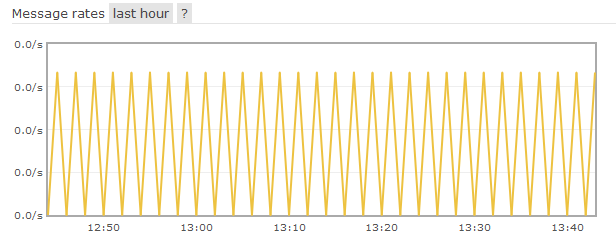
\includegraphics[scale=0.7]{rate-rabbit-mq-heartbeat.png}
            \caption{Mensajes por hora - HeartBeat}
            \label{fig:rabbitmq-rate-heartbeat}
        \end{figure}
        
        \begin{figure}[H]
        \centering
            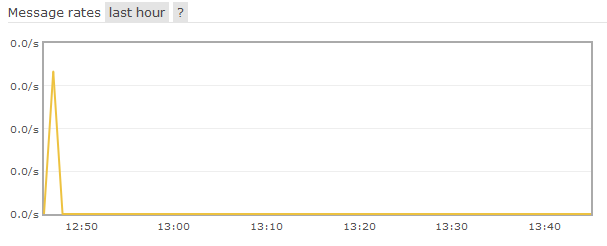
\includegraphics[scale=0.7]{rate-rabbit-mq-updates.png}
            \caption{Mensajes por hora - Updates}
            \label{fig:rabbitmq-rate-updates}
        \end{figure}
        
        En la tabla \ref{tab:test-results} se muestran los resultados obtenidos por parte de la aplicación durante el proceso de pruebas de funcionamiento. El campo ``Ejecución'' indica el comando ejecutado para la realización de la prueba, mientras que las ``Condiciones especiales'' hacen referencia a restricciones que se han aplicado y que no pueden ser mostradas de otra forma. 

        \begin{table}[H]             
            \centering                  
                \resizebox{\textwidth}{!}{   
                    \begin{tabular}{lllll}
                        \hline
                        \textbf{Ejecución}                          &   \textbf{Condiciones especiales}         &   \textbf{R. esperado}    &   \textbf{R. obtenido}    &   \textbf{R. pruebas}       \\
                        \hline
                         run                                        &   Ninguna                                 &   Éxito                   &   Éxito                   &   Éxito                     \\
                         run                                        &   Agente iniciado como servicio           &   Éxito                   &   Éxito                   &   Éxito                     \\
                         run                                        &   Archivo de configuración no existente   &   Éxito                   &   Éxito                   &   Éxito                     \\
                         run -i heartbeat                           &   Ninguna                                 &   Éxito                   &   Éxito                   &   Éxito                     \\
                         run config.json                            &   Archivo de configuración no existente   &   Éxito                   &   Éxito                   &   Éxito                     \\
                         run -i heartbeat                           &   \textit{Plugin} no existente            &   Fallo                   &   Fallo                   &   Éxito                     \\
                         run config.json                            &   Ninguna                                 &   Fallo                   &   Fallo                   &   Éxito                     \\
                         run --output-options outputType:table      &   Ninguna                                 &   Éxito                   &   Éxito                   &   Éxito                     \\
                         run --output-options outputType=table      &   Ninguna                                 &   Fallo                   &   Fallo                   &   Éxito                     \\
                         run --output-options outputType:image      &   Ninguna                                 &   Éxito                   &   Éxito                   &   Éxito                     \\
                         service --install                          &   Ninguna                                 &   Éxito                   &   Éxito                   &   Éxito                     \\
                         service --install                          &   Agente ya instalado                     &   Fallo                   &   Fallo                   &   Éxito                     \\
                         service --uninstall                        &   Ninguna                                 &   Éxito                   &   Éxito                   &   Éxito                     \\
                         service --uninstall                        &   Agente no instalado                     &   Fallo                   &   Fallo                   &   Éxito                     \\
                         service --uninstall                        &   Agente en ejecución                     &   Fallo                   &   Fallo                   &   Éxito                     \\
                         service --start                            &   Ninguna                                 &   Éxito                   &   Éxito                   &   Éxito                     \\
                         service --start                            &   Agente no instalado                     &   Fallo                   &   Fallo                   &   Éxito                     \\
                         service --start                            &   Agente en ejecución                     &   Fallo                   &   Fallo                   &   Éxito                     \\
                         service --stop                             &   Ninguna                                 &   Éxito                   &   Éxito                   &   Éxito                     \\
                         service --stop                             &   Agente no instalado                     &   Fallo                   &   Fallo                   &   Éxito                     \\
                         service --stop                             &   Agente no iniciado                      &   Fallo                   &   Fallo                   &   Éxito                     \\
                        \hline&
                    \end{tabular}
                }
            \caption{Resultados de las pruebas}
            \label{tab:test-results}
        \end{table}